\documentclass[tikz,border=3pt]{standalone}
\usepackage{amsmath}
\usepackage{xcolor}
\usetikzlibrary{arrows.meta,positioning,fit,calc}
\definecolor{semcol}{HTML}{5B3CC4}
\definecolor{auditcol}{HTML}{E56717}
\definecolor{govcol}{HTML}{2E7D32}
\definecolor{hostcol}{HTML}{37474F}
\definecolor{bandcol}{HTML}{2F5DA8}
\begin{document}
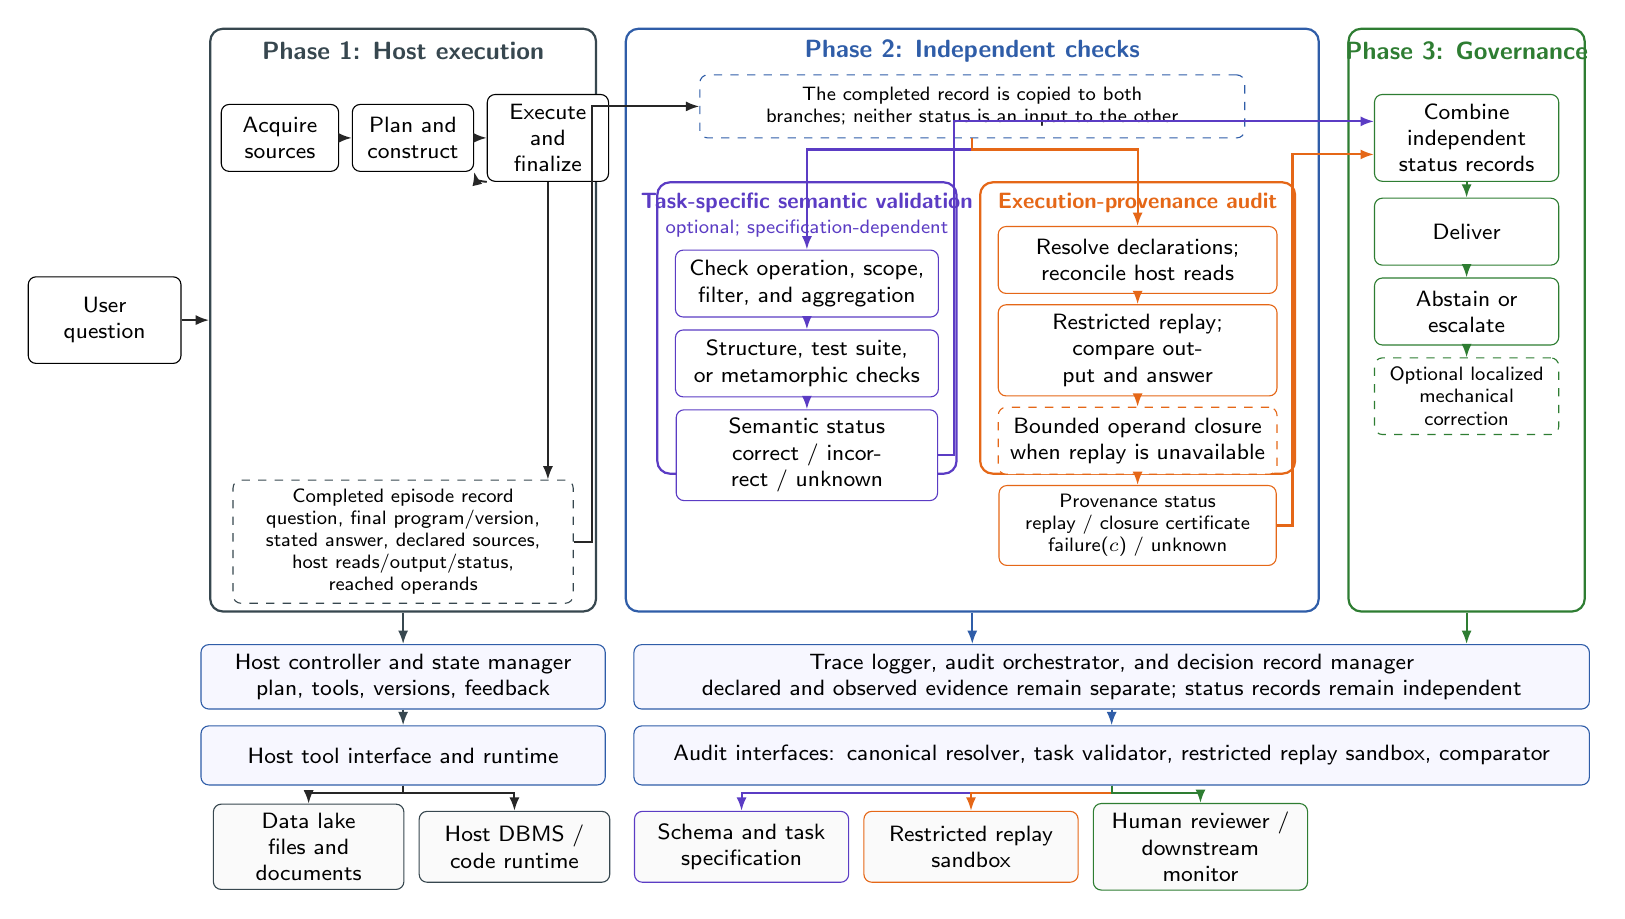
\begin{tikzpicture}[
  font=\sffamily\footnotesize,
  >={Latex[length=1.7mm]},
  flow/.style={->,line width=.7pt,draw=black!85},
  cflow/.style={->,line width=.75pt},
  optflow/.style={->,line width=.65pt,dashed,draw=govcol},
  phase/.style={draw,rounded corners=1.6mm,line width=.8pt,inner sep=1.8mm,fill=white},
  stepbox/.style={draw,rounded corners=1mm,align=center,minimum height=8.5mm,inner sep=1.2mm,fill=white},
  status/.style={draw,rounded corners=1mm,align=center,minimum height=8mm,inner sep=1.1mm,fill=white},
  band/.style={draw=bandcol,rounded corners=1mm,align=center,minimum height=7.5mm,fill=blue!3},
  resource/.style={draw,rounded corners=1mm,align=center,minimum height=9mm,inner sep=1.1mm,fill=gray!4},
  title/.style={font=\sffamily\bfseries\small},
  branchtitle/.style={font=\sffamily\bfseries\footnotesize},
  note/.style={font=\sffamily\scriptsize,align=center}
]

% Input and Phase 1
\node[stepbox,text width=17mm,minimum height=11mm] (q) {User\\question};
\node[phase,draw=hostcol,minimum width=49mm,minimum height=74mm,right=3.5mm of q] (p1) {};
\node[title,text=hostcol] at ($(p1.north)+(0,-3mm)$) {Phase 1: Host execution};
\node[stepbox,text width=12.5mm] (acq) at ($(p1.north west)+(9mm,-14mm)$) {Acquire\\sources};
\node[stepbox,text width=13mm,right=1.6mm of acq] (build) {Plan and\\construct};
\node[stepbox,text width=13mm,right=1.6mm of build] (exec) {Execute and\\finalize};
\draw[flow] (q)--(p1.west|-q);
\draw[flow] (acq)--(build); \draw[flow] (build)--(exec);
\draw[flow,bend left=38] (exec.south west) to (build.south east);
\node[status,draw=hostcol,dashed,text width=41mm,font=\sffamily\scriptsize] (episode) at ($(p1.south)+(0,9mm)$) {Completed episode record\\question, final program/version, stated answer, declared sources, host reads/output/status, reached operands};
\draw[flow] (exec.south) -- (episode.north -| exec.south);

% Phase 2 shell
\node[phase,draw=bandcol,minimum width=88mm,minimum height=74mm,right=3.5mm of p1] (p2) {};
\node[title,text=bandcol] at ($(p2.north)+(0,-3mm)$) {Phase 2: Independent checks};
\node[status,draw=bandcol,dashed,text width=67mm,font=\sffamily\scriptsize] (record) at ($(p2.north)+(0,-10mm)$) {The completed record is copied to both branches; neither status is an input to the other};
\draw[flow] (episode.east) -- ++(2.3mm,0) |- (record.west);

% Semantic branch
\node[phase,draw=semcol,minimum width=38mm,minimum height=37mm] (sem) at ($(p2.center)+(-21mm,-1mm)$) {};
\node[branchtitle,text=semcol] at ($(sem.north)+(0,-2.7mm)$) {Task-specific semantic validation};
\node[note,text=semcol] at ($(sem.north)+(0,-6mm)$) {optional; specification-dependent};
\node[stepbox,draw=semcol,text width=31mm] (sem1) at ($(sem.north)+(0,-13mm)$) {Check operation, scope,\\filter, and aggregation};
\node[stepbox,draw=semcol,text width=31mm,below=1.5mm of sem1] (sem2) {Structure, test suite,\\or metamorphic checks};
\node[status,draw=semcol,text width=31mm,below=1.5mm of sem2] (semstat) {Semantic status\\correct / incorrect / unknown};
\draw[cflow,draw=semcol] (sem1)--(sem2); \draw[cflow,draw=semcol] (sem2)--(semstat);
\draw[cflow,draw=semcol] (record.south) -- ++(0,-1.4mm) -| (sem1.north);

% Provenance branch
\node[phase,draw=auditcol,minimum width=40mm,minimum height=37mm] (aud) at ($(p2.center)+(21mm,-1mm)$) {};
\node[branchtitle,text=auditcol] at ($(aud.north)+(0,-2.7mm)$) {Execution-provenance audit};
\node[stepbox,draw=auditcol,text width=33mm] (aud1) at ($(aud.north)+(0,-10mm)$) {Resolve declarations;\\reconcile host reads};
\node[stepbox,draw=auditcol,text width=33mm,below=1.3mm of aud1] (aud2) {Restricted replay;\\compare output and answer};
\node[stepbox,draw=auditcol,dashed,text width=33mm,below=1.3mm of aud2] (aud3) {Bounded operand closure\\when replay is unavailable};
\node[status,draw=auditcol,text width=33mm,below=1.3mm of aud3,font=\sffamily\scriptsize] (audstat) {Provenance status\\replay / closure certificate\\failure($c$) / unknown};
\draw[cflow,draw=auditcol] (aud1)--(aud2); \draw[cflow,draw=auditcol] (aud2)--(aud3); \draw[cflow,draw=auditcol] (aud3)--(audstat);
\draw[cflow,draw=auditcol] (record.south) -- ++(0,-1.4mm) -| (aud1.north);

% Phase 3
\node[phase,draw=govcol,minimum width=30mm,minimum height=74mm,right=3.5mm of p2] (p3) {};
\node[title,text=govcol,align=center] at ($(p3.north)+(0,-3mm)$) {Phase 3: Governance};
\node[stepbox,draw=govcol,text width=21mm] (combine) at ($(p3.north)+(0,-14mm)$) {Combine independent\\status records};
\node[stepbox,draw=govcol,text width=21mm,below=2mm of combine] (deliver) {Deliver};
\node[stepbox,draw=govcol,text width=21mm,below=1.5mm of deliver] (abstain) {Abstain or\\escalate};
\node[stepbox,draw=govcol,dashed,text width=21mm,below=1.5mm of abstain,font=\sffamily\scriptsize] (repair) {Optional localized\\mechanical correction};
\draw[cflow,draw=semcol] (semstat.east) -- ++(2mm,0) |- ($(combine.west)+(0,2.1mm)$);
\draw[cflow,draw=auditcol] (audstat.east) -- ++(2mm,0) |- ($(combine.west)+(0,-2.1mm)$);
\draw[cflow,draw=govcol] (combine)--(deliver); \draw[cflow,draw=govcol] (deliver)--(abstain); \draw[optflow] (abstain)--(repair);

% Lower layers
\node[band,text width=49mm,below=4mm of p1] (hostctl) {Host controller and state manager\\plan, tools, versions, feedback};
\node[band,text width=119mm,right=3.5mm of hostctl] (auditctl) {Trace logger, audit orchestrator, and decision record manager\\declared and observed evidence remain separate; status records remain independent};
\node[band,text width=49mm,below=2mm of hostctl] (hostif) {Host tool interface and runtime};
\node[band,text width=119mm,right=3.5mm of hostif] (auditif) {Audit interfaces: canonical resolver, task validator, restricted replay sandbox, comparator};

\node[resource,draw=hostcol,text width=22mm,below=2.3mm of hostif,xshift=-12mm] (lake) {Data lake\\files and documents};
\node[resource,draw=hostcol,text width=22mm,right=1.8mm of lake] (db) {Host DBMS /\\code runtime};
\node[resource,draw=semcol,text width=25mm,right=3mm of db] (spec) {Schema and task\\specification};
\node[resource,draw=auditcol,text width=25mm,right=1.8mm of spec] (sandbox) {Restricted replay\\sandbox};
\node[resource,draw=govcol,text width=25mm,right=1.8mm of sandbox] (human) {Human reviewer /\\downstream monitor};

\draw[cflow,draw=hostcol] (p1.south)--(hostctl.north); \draw[cflow,draw=hostcol] (hostctl)--(hostif);
\draw[cflow,draw=bandcol] (p2.south)--(auditctl.north -| p2.south); \draw[cflow,draw=govcol] (p3.south)--(auditctl.north -| p3.south);
\draw[cflow,draw=bandcol] (auditctl)--(auditif);
\draw[flow] (hostif.south) -- ++(0,-1mm) -| (lake.north); \draw[flow] (hostif.south) -- ++(0,-1mm) -| (db.north);
\draw[cflow,draw=semcol] (auditif.south) -- ++(0,-1mm) -| (spec.north);
\draw[cflow,draw=auditcol] (auditif.south) -- ++(0,-1mm) -| (sandbox.north);
\draw[cflow,draw=govcol] (auditif.south) -- ++(0,-1mm) -| (human.north);
\end{tikzpicture}
\end{document}
